\chapter[Introdução]{Introdução}
\label{cap:intro}

IoT é um conceito que vem ganhado força ao longo dos anos, graças ao estudo, prototipação e desenvolvimento de diversas protocolos e tecnologias. Os pontos chave para o seu desenvolvimento foram a miniaturização de processadores e sensores; melhoramento de baterias e otimização do uso destas; definição de novos protocolos de rede; e aumento da robustez de protocolos de comunicação sem-fio.

A Internet das Coisas, representado na figura \ref{fig:iotimg}, mais conhecida pelo seu acrônimo em inglês IoT(\textit{Internet of Things}), foi cunhada pelo engenheiro britânico Kevin Ashton no final dos anos 1990 onde ele, trabalhando para a P\&G, pensou na possibilidade de que os produtos da empresa estivessem munidos de identificadores e capazes de estabelecer comunicação através da Internet, que na época estava se estabelecendo, criando assim uma rede onde as coisas estivessem conectadas \cite{KA_IOT}. Assim, os computadores se tornariam capazes de rastrear e identificar tudo, podendo reduzir desperdícios, minimizar custos e identificar o momento certo quando substituir ou reparar um produto \cite{lopezIOT}.

\begin{figure}[ht]
    \centering
    \caption{Internet of Things (IoT)}
    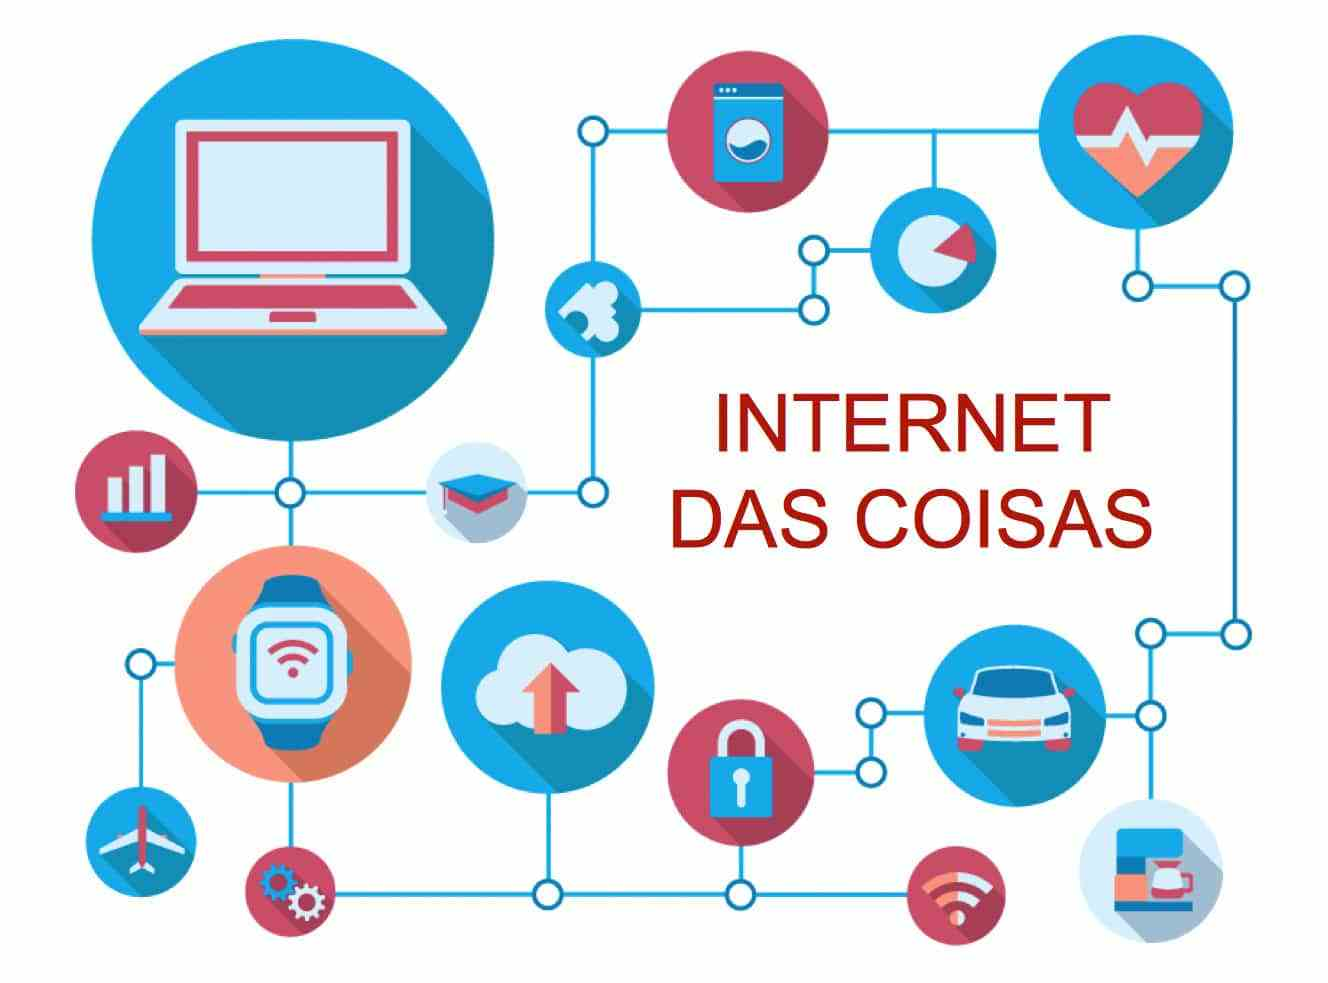
\includegraphics[width=10cm]{./sections/textual/chapters/images/intro_iot.jpg}\\
    Retirado do site http://sentrybrasil.com.br/cursos/internet-das-coisas-vai-revolucionar-o-mercado/
    \label{fig:iotimg}
\end{figure}


Atualmente há diversas aplicações de IoT, desde implementações em larga escala como cidades inteligentes conforme descrito em \cite{sotres2017practical}, onde em Santander na Espanha é implantado por toda a cidade nós com múltiplos sensores afim de disponibilizar uma plataforma de testes. Aplicações de \emph{smart campus} como apresentada em \cite{wang2017performance} que mostra a aplicação de uma rede de sensores sem fio para verificar a qualidade do ar. Aplicações de saúde como em \cite{zhang2015remote}, onde é coletado e analisado em tempo real informações de pressão sanguínea e peso corporal do paciente, sendo estes dados utilizados para verificar a probabilidade do paciente ter um evento de insuficiência cardíaca, utilizando técnicas de aprendizado de maquina.

% Após o termo ser cunhado em 1999, foram necessários anos de evolução tecnológica para a atual popularidade do conceito. Por exemplo, a criação da plataforma de desenvolvimento de hardware aberta Arduino em 2005 \cite{OC_ARDUINO}, tornou fácil o estudo e a prototipação de itens de baixo custo. \ff{adicionar exemplos como o IPv6, baterias e os protocolos de Sem Fio}

A implementação de uma aplicação IoT necessita de uma rede de nós sensores distribuídas geralmente conectadas a um nó central, conhecido como nó gateway, que tem por finalidade encaminhar os dados coletados para processamento. Para tal implementação existem duas abordagens clássicas: conexões cabeadas entre os nós da rede e a utilização de redes sem fio \cite{gomes2017estimaccao}. Como vantagem em relação às redes sem fio, as conexões cabeadas apresentam maior confiabilidade na conexão. Em contrapartida, a utilização de redes sem fio se destaca, em relação à redes cabeadas, nos quesitos de flexibilidade, custo de implantação, facilidade e rápidez na implementação e na manutenção \cite{gungor2009industrial}.

As vantagens que Redes de Sensores Sem Fio(RSSF), representado na figura \ref{fig:rssf}, apresentam, fazem estas se destacarem na implementação de aplicações IoT, há porém ainda desafios para uma implementação robusta de comunicações sem fio, pois o meio de transmissão é caótico e pouco confiável. Interferências, ruídos, sombreamento e propagação por multi percurso no meio podem ocasionar altas taxas de perda de pacote e alta latência \cite{gomes2017estimaccao}.

\begin{figure}[ht]
    \begin{center}
        \caption{RSSF - Topologia Estrela}
        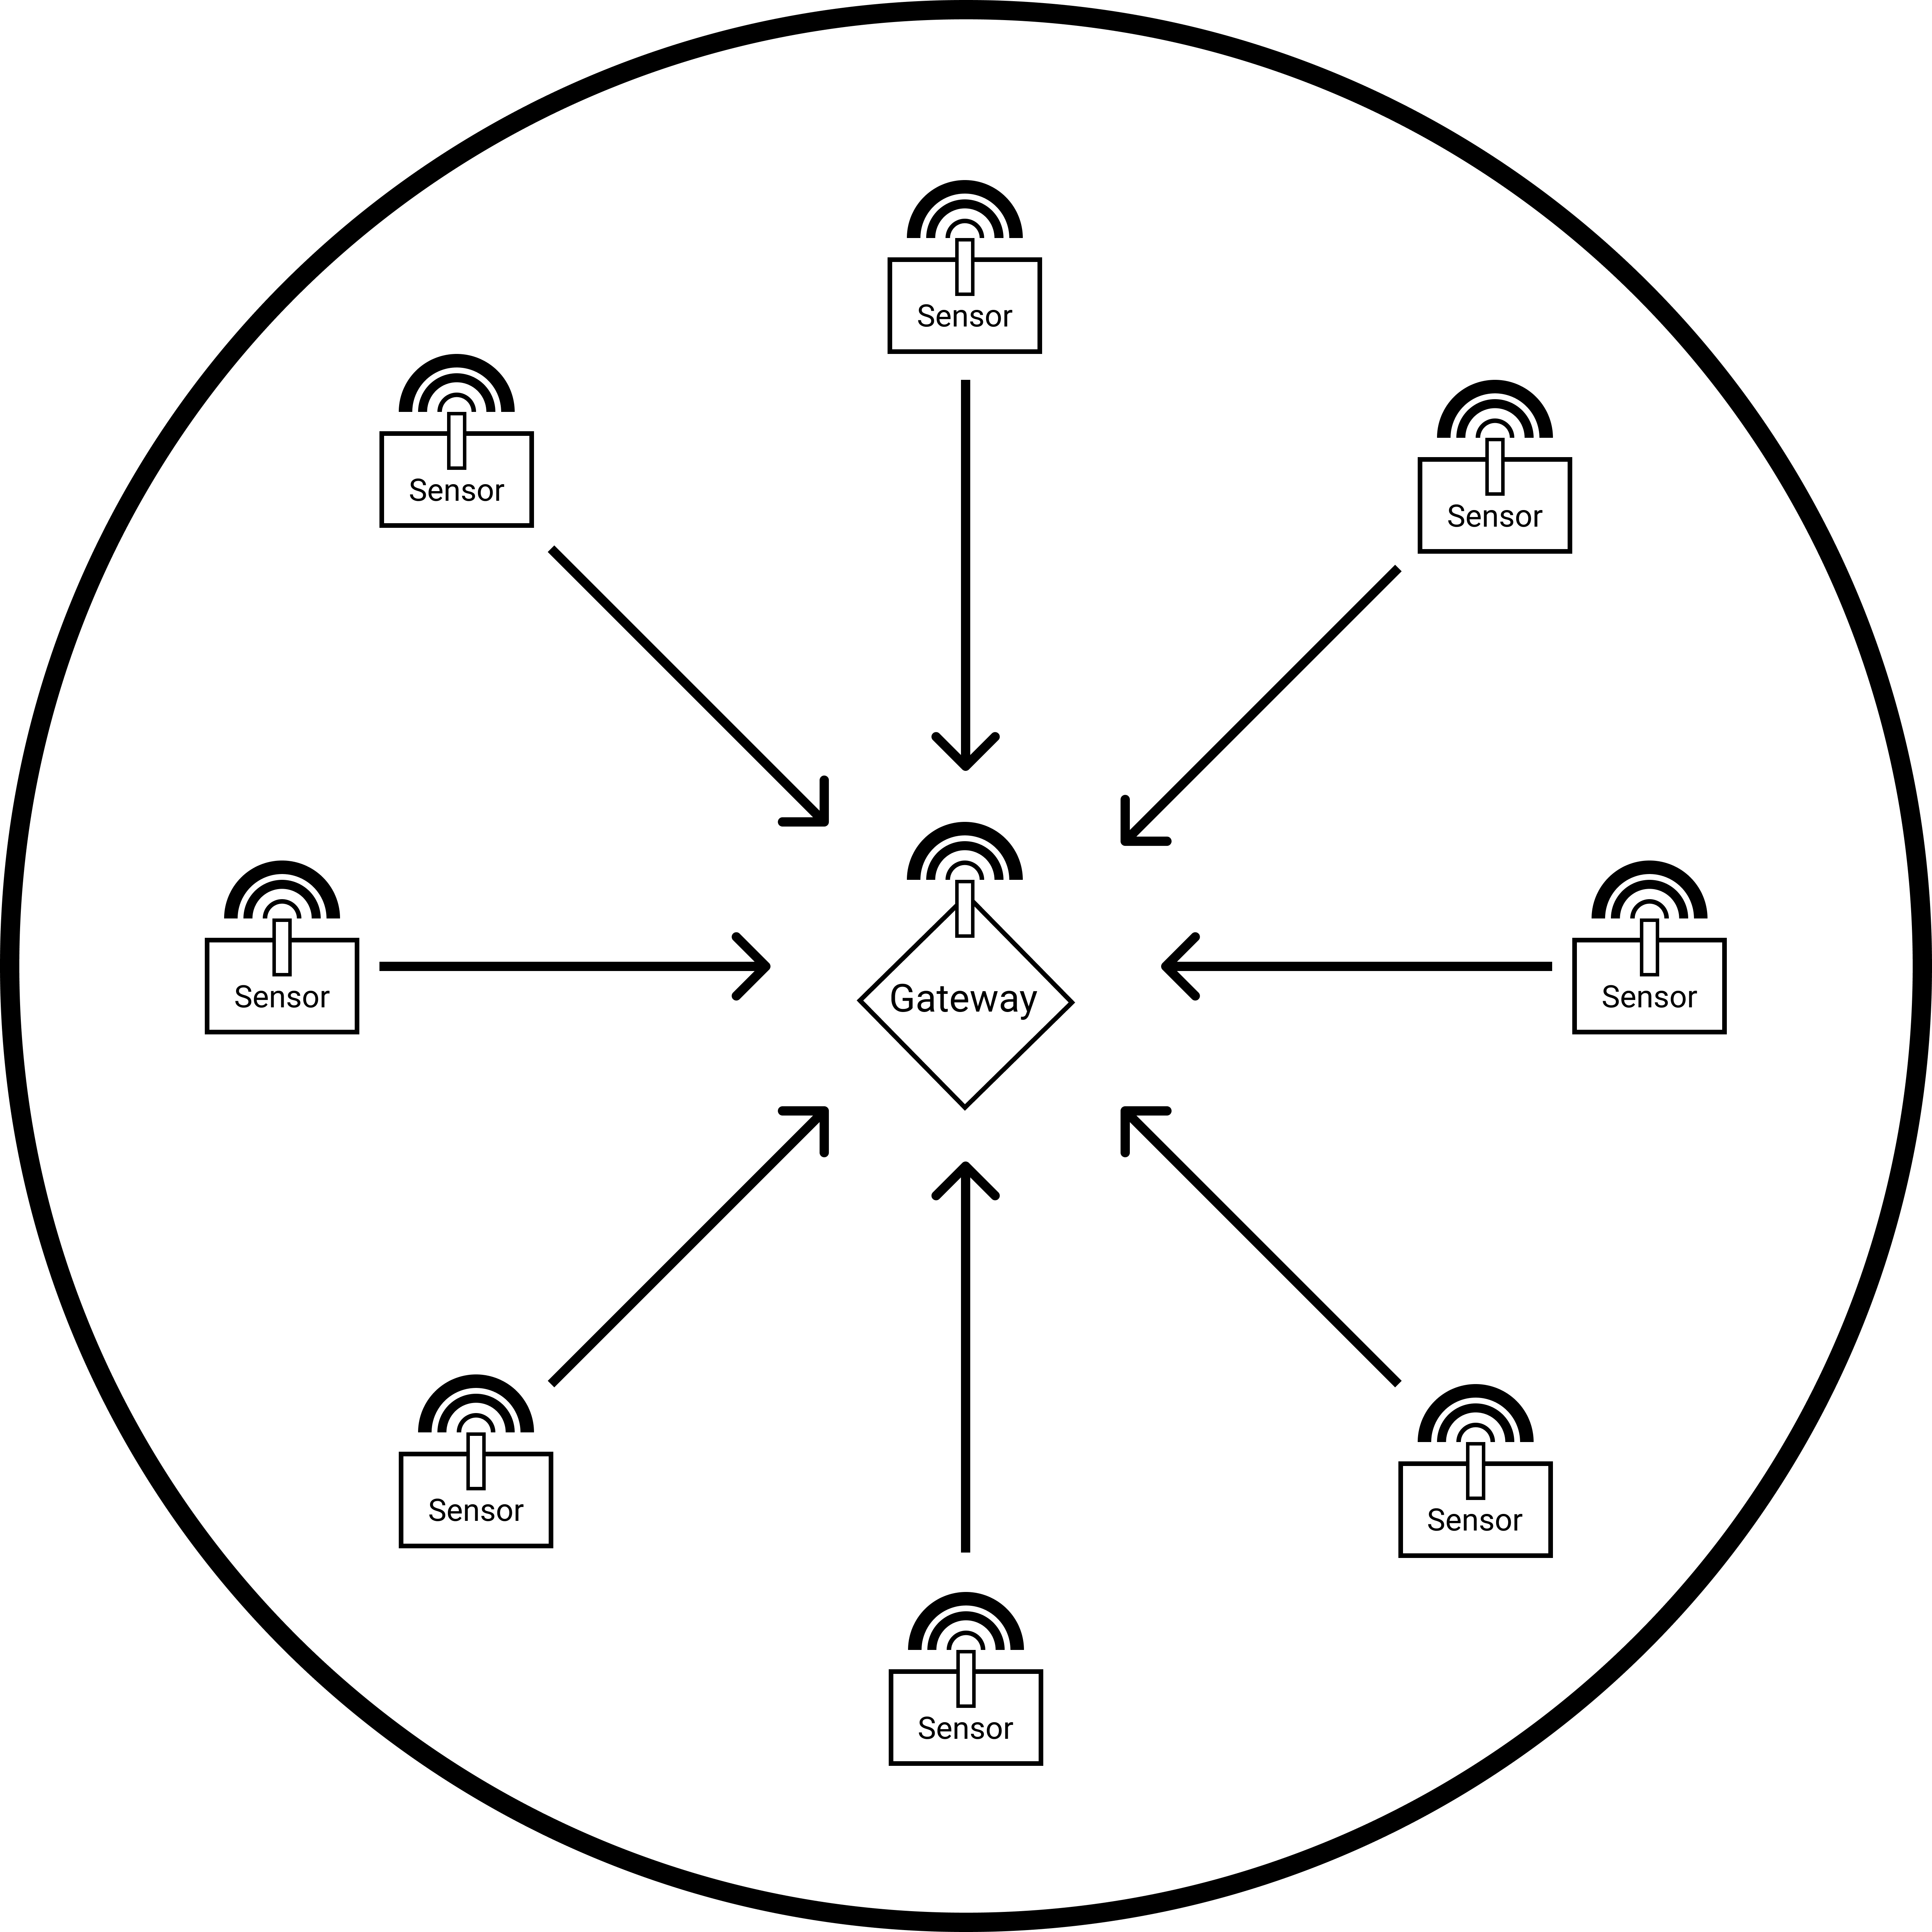
\includegraphics[width=10cm]{./sections/textual/chapters/images/intro_rssf.png}\\
        Fonte autoral
        \label{fig:rssf}
    \end{center}
\end{figure}

Para contornar os desafios da comunicação sem fio, padrões e tecnologias foram desenvolvidos. Um dos principais órgãos na padronização em telecomunicações é o Instituto de Engenheiros Eletricistas e Eletrônicos, Institute of Electrical and Electronics Engineers, mais conhecido pela sigla IEEE. Por exemplo, para redes locais o Wi-Fi, baseado no padrão IEEE 802.11, se tornou uma tecnologia confiável que pode apresentar altas taxas de transferência com uma latência baixa. Em redes de curto alcance, o Bluetooth, baseado no padrão IEEE 802.15.1, se tornou trivial na vida das pessoas através do uso para conexão de fones de ouvido, teclados e mouses sem fio. Estes padrões, apesar de já bem estabelecidos no mercado, possuem alguns problemas para o desenvolvimento de RSSF, que geralmente requerem múltiplos dispositivos espalhados e, principalmente, sem acesso fácil a uma fonte continua de energia.

Tendo em vista este problema energético, alguns padrões foram desenvolvidos para oferecer uma comunicação de qualidade e focando em eficiência energética para a utilização de baterias. Iniciativas privadas desenvolveram, por exemplo, o SigFox e LoRa. O IEEE desenvolveu o padrão 802.15.4 e o aprimorou ao longo dos anos com adição de emendas, que foram responsáveis pelo desenvolvimento de aplicações como ZigBee e Wi-SUN. A \emph{3rd Generation Partnership Project}(3GPP) Projeto de Parceria de terceira geração em tradução livre, desenvolveu a tecnologia NB-IoT, uma versão simplificada do LTE que visa utilizar a mesma infraestrutura porém com uma melhor eficiência energética. Estas tecnologias podem ser utilizadas para a implementação de redes classificadas como Redes de Longo Alcance e Baixo Consumo Energético.

\section{Justificativa e Relevância do Trabalho}
\label{sec:justificativa}
Em \cite{tuset2020dataset} os autores implementaram uma RSSF utilizando as modulações propostas na emenda ``g'' do padrão IEEE 802.15.4. Este experimento foi realizado em um cenário industrial, durando um total de 99 dias gerando um conjunto de dados que foi utilizado para averiguar a confiabilidade da rede. Os dados foram analisados e utilizados para propor mecanismos de diversidade de modulação que, como mostrado em \cite{gomes2020improving}, pode melhorar a taxa de entrega de pacotes.

O cenário industrial apresenta diversos problemas, principalmente relacionados à interferência e propagação multi-caminho. Diferentes ambientes possuem diferentes problemas em relação a comunicação via rádio. Então, pensando em analisar os efeitos da propagação de ondas de rádio em outro cenário, este trabalho então se propõe a analisar a comunicação sem fio de transceptores do padrão IEEE 802.15.4g SUN em um ambiente predial, também denominado neste texto como \emph{Smart Building}, que possui como maior fonte de problemas para a comunicação a falta de linha de visada. Estudando o comportamento da RSSF a partir da verificação da taxa de entrega de pacotes. E portanto, analisando a viabilidade da rede a partir da tecnologia utilizada.

\section{Objetivos}
\label{sec:objetivos}

\subsection{Objetivo Geral}
\label{subsec:objGeral}
Implantar uma RSSF e coletar as informações das transmissões realizadas através das modulações definidas pelo padrão IEEE 802.15.4g e analisar o comportamento destas no cenário de \emph{Smart Building}.

% Coletar e analisar os dados experimentais de transmissões realizadas entre os dispositivos openmote que implementam as modulações definidas no padrão IEEE 802.15.4g SUN espalhados pelo prédio dos professores no campus Campina Grande.

\subsection{Objetivos Específicos}
\label{subsec:objespecificos}
\begin{itemize}
    \item Implementar uma rede sem fio utilizando transceptores das modulações do IEEE 802.15.4g;
    \item Coletar, armazenar e disponibilizar os dados relativas as transmissões realizadas;
    \item Analisar os dados e gerar informações a respeito da comunicação entre dispositivos neste cenário.
\end{itemize}


\section{Metodologia}
\label{sec:metodologia}
Para alcançar os objetivos acima, foram realizados os seguintes passos:

% Estudei a plataforma de desenvolvimento do Openmote
% Fiz as mudanças no código de Pere
% fiz o código python dos gateways/persistência dos dados no influx
% Colocar pra rodar o experimento
% analise dos dados

\begin{itemize}
    \item \refact{Estudo e implementação dos dispositivos: Os dispositivos utilizados neste projeto possuem o código disponível em um repositório github \cite{pere2019}. Bem como algumas alterações no código fonte para esta aplicação;}
    \item \refact{Persistência dos dados: Desenvolvimento de um script responsável por coletar e persistir os dados gerados em um banco de dados InfluxDB;}
    \item \refact{Execução do experimento: Distribuição dos nós transmissores pelo prédio e instalação dos softwares e scripts necessarios para persistencia dos dados;}
    \item \refact{Análise dos resultados: A partir dos dados coletados e salvos localmente, foram feitas analises e gerado informações as quais estarão na seção de resultados.}
\end{itemize}

\section{Organização do Documento}
\label{sec:organizacao}
\todo{A ser feito quando o documento tiver pronto}